\begin{figure}[H]
    \centering
    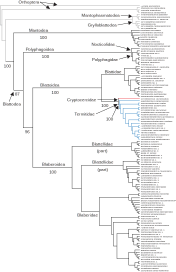
\includegraphics[scale=0.7]{images/inward_phyl.pdf}
    \vspace{0.5cm}
    \mycaption{Topology of Bayesian majority rules consensus tree of 2501 trees from \citet{inwardDeathOrderComprehensive2007}}{Red branch indicates position of \textit{Cryptocercus}, blue branches indicate termite lineage. Numbers under the branches indicate posterior probabilities (i.e. the proportion of the 2501 sampled trees that contain the node) for key nodes. Names of major clades (e.g superfamilies) are provisional.}
\end{figure}

\pagebreak
\begin{figure}[H]
    \centering
    \includegraphics[scale=0.9]{images/evangelista2019.pdf}
    \vspace{0.5cm}
    \mycaption{Time-calibrated phylogeny of Blattodea from \citet{evangelistaIntegrativePhylogenomicApproach2019}.}{Topology obtained from ML analysis of the decisive amino acid (aa) dataset (585 040 aa positions). Coloured circles represent BS support. Node dates (posterior mean) were inferred using the decisive aa dataset reduced to sites containing 95\% or more data completeness, and nine
    exhaustively vetted fossil calibrations. Error bars represent 95\% confidence intervals. Fossils used for calibrations indicated as numbers in black circles are: 1: \textit{Cretaholocompsa montespan}; 2: \textit{Archeorhinotermes rossi}; 3: \textit{Valditermes brenanae}; 4: \textit{‘Gyna’ obesa}; 5: \textit{Qilianiblatta namurensis}; 6: \textit{Juramantophasma sinica}; 7: \textit{Alexarasnia rossica}; 8: \textit{Raphogla rubra}; 9: \textit{Protelytron permianum}.}
    \label{fig:evangelista}
\end{figure}

\pagebreak
\csvreader[
longtable=lllll,
table head=
    \mycaption{A very long but beautiful table}{for the analysis with respective \textsc{GenBank}-ID's.} \label{tab:species}\\
    \toprule \bfseries No &\bfseries Order &\bfseries Family &\bfseries Species &\bfseries GenBankID \\ \midrule\endfirsthead\\ 
    \toprule \bfseries No &\bfseries Order &\bfseries Family &\bfseries Species &\bfseries GenBankID \\ \midrule\endhead \bottomrule\endfoot,
late after line=\\,
before reading={\catcode`\#=12},
after reading={\catcode`\#=6},
]{appendix/species.csv}{1=\No,2=\Order,3=\Family,4=\Species, 5=\GenBankID}{\No & \Order & \Family & \Species & \GenBankID}
